% This is LLNCS.DEM the demonstration file of
% the LaTeX macro package from Springer-Verlag
% for Lecture Notes in Computer Science,
% version 2.4 for LaTeX2e as of 16. April 2010
%
\documentclass{llncs}

% allows for temporary adjustment of side margins
\usepackage{chngpage}

% just makes the table prettier (see \toprule, \bottomrule, etc. commands below)
\usepackage{booktabs}

\usepackage[utf8]{inputenc}
%\usepackage[font=small,skip=0pt]{caption}

% footnotes
\usepackage{scrextend}

% URL handling
\usepackage{url}
\urlstyle{same}

% Todos
%\usepackage[colorinlistoftodos]{todonotes}
%\newcommand{\ke}[1]{\todo[size=\small, color=orange!40]{\textbf{Kai:} #1}}
%\newcommand{\tb}[1]{\todo[size=\small, color=green!40]{\textbf{Thomas:} #1}}


%\usepackage{makeidx}  % allows for indexgeneration

%\usepackage{amsmath}
\usepackage{amsmath, amssymb}
\usepackage{mathabx}

% monospace within text
\newcommand{\ms}[1]{\texttt{#1}}

% examples
\usepackage{fancyvrb}
\DefineVerbatimEnvironment{ex}{Verbatim}{numbers=left,numbersep=2mm,frame=single,fontsize=\scriptsize}

\usepackage{xspace}
% Einfache und doppelte Anfuehrungszeichen
\newcommand{\qs}{``} 
\newcommand{\qe}{''\xspace} 
\newcommand{\sqs}{`} 
\newcommand{\sqe}{'\xspace} 

% checkmark
\usepackage{tikz}
\def\checkmark{\tikz\fill[scale=0.4](0,.35) -- (.25,0) -- (1,.7) -- (.25,.15) -- cycle;} 

% Xs
\usepackage{pifont}

% Tabellenabstände kleiner
\setlength{\intextsep}{10pt} % Vertical space above & below [h] floats
\setlength{\textfloatsep}{10pt} % Vertical space below (above) [t] ([b]) floats
% \setlength{\abovecaptionskip}{0pt}
% \setlength{\belowcaptionskip}{0pt}

\usepackage{tabularx}
\newcommand{\hr}{\hline\noalign{\smallskip}} % für die horizontalen linien in tabellen

% Todos
\usepackage[colorinlistoftodos]{todonotes}
\newcommand{\ke}[1]{\todo[size=\small, color=orange!40]{\textbf{Kai:} #1}}
\newcommand{\tb}[1]{\todo[size=\small, color=green!40]{\textbf{Thomas:} #1}}
\newcommand{\er}[1]{\todo[size=\small, color=red!40]{\textbf{Erman:} #1}}
\newcommand{\an}[1]{\todo[size=\small, color=blue!40]{\textbf{Andy:} #1}}

\newenvironment{table-1cols}{
  \scriptsize
  \sffamily
  \vspace{0.3cm}
  \begin{tabular}{l}
  \hline
  \textbf{Requirements} \\
  \hline

}{
  \hline
  \end{tabular}
  \linebreak
}

\newenvironment{table-2cols}{
  \scriptsize
  \sffamily
  \vspace{0.3cm}
  \begin{tabular}{l|l}
  \hline
  \textbf{Requirements} & \textbf{Covering DSCLs} \\
  \hline

}{
  \hline
  \end{tabular}
  \linebreak
}

\newenvironment{complexity}{
  %\scriptsize
  %\sffamily
  %\vspace{0.3cm}
  \begin{tabular}{l|l}
  \hline
  \textbf{Complexity Class} & \textbf{Complexity} \\
  \hline

}{
  \hline
  \end{tabular}
  \linebreak
}

\newenvironment{DL}{
  %\scriptsize
  %\sffamily
  \vspace{0cm}
  \begin{tabular}{r l}

}{
  \end{tabular}
  %\linebreak
}


\newenvironment{evaluation}{
  %\scriptsize
  %\sffamily
  %\vspace{0.3cm}
  \begin{tabular}{l|c|c|c|c|c|c}
  \hline
  \textbf{Constraint Class} & \textbf{DSP} & \textbf{OWL2-DL} & \textbf{OWL2-QL} & \textbf{ReSh} & \textbf{ShEx} & \textbf{SPIN} \\
  \hline

}{
  \hline
  \end{tabular}
  \linebreak
}

\newenvironment{constraint-languages-complexity}{
  %\scriptsize
  %\sffamily
  %\vspace{0.3cm}
  \begin{tabular}{l|c|c|c|c|c|c}
  \hline
  \textbf{Complexity Class} & \textbf{DSP} & \textbf{OWL2-DL} & \textbf{OWL2-QL} & \textbf{ReSh} & \textbf{ShEx} & \textbf{SPIN} \\
  \hline

}{
  \hline
  \end{tabular}
  \linebreak
}

\newenvironment{user-fiendliness}{
  %\scriptsize
  %\sffamily
  %\vspace{0.3cm}
  \begin{tabular}{l|c|c|c|c|c}
  \hline
  \textbf{criterion} & \textbf{DSP} & \textbf{OWL2} & \textbf{ReSh} & \textbf{ShEx} & \textbf{SPIN} \\
  \hline

}{
  \hline
  \end{tabular}
  \linebreak
}

\setcounter{secnumdepth}{5}

\begin{document}

%
%
\title{RDF Validation}
\subtitle{Classification of Constraints and Constraint Languages According to Reasoning, Expressivity, and Complexity}
%
\titlerunning{XXXXX}  % abbreviated title (for running head)
%                                     also used for the TOC unless
%                                     \toctitle is used
%
\author{Thomas Bosch\inst{1} \and Erman Acar\inst{2} \and Andreas Nolle\inst{3} \and Christian Meilicke\inst{2} \and Kai Eckert\inst{2}}
%
\authorrunning{XXXXX} % abbreviated author list (for running head)
%
%%%% list of authors for the TOC (use if author list has to be modified)
\institute{GESIS – Leibniz Institute for the Social Sciences, Germany\\
\email{thomas.bosch@gesis.org},\\ 
\and
University of Mannheim, Germany \\
\email{\{christian,erman,kai\}@informatik.uni-mannheim.de} 
\and
Albstadt-Sigmaringen University, Germany \\
\email{nolle@hs-albsig.de}
}

\maketitle              % typeset the title of the contribution

\begin{abstract}
There is no standard way to formulate RDF constraints and to validate data according to these constraints,
although there are five promising constraint languages covering all requirements on RDF validation.
The ontology language OWL 2 can be used as an expressive constraint language with a high level human-readable syntax.
We explain why OWL 2 reasoning is beneficial for validation and how reasoning interacts with validation.
%We take reasoning into account as a possible pre-validation step, 
%(1) to infer triples resolving constraint violations, 
%(2) to infer triples for which constraints can also be validated, and 
%(3) to solve the major shortcoming of RDF validation: redundancy. 
%\er{I simplified the long abstract a bit by commenting (\%) as well as little editing. The part starting with, "we investigate", cause lacking integrity in abstract,  I dropped 1, 2, 3 for simplification and better flow. We can write abstract in the end, which can also include a short part of introduction if necessary.}
We also attempt to classify the expressivity, the complexity, and the user-friendliness of constraint languages. 
Following this approach, one can clarify which constraint language to use to express constraints for specific validation scenarios, with and without reasoning concerning the complexity as well as user-friendliness.
%Validators can determine which axioms cause high complexity and which constraints can only be expressed within a more sophisticated expressivity class.
%As a next step, validators give some guidance how to get to lower expressivity and complexity classes.
%If validators propose multiple constraint languages for a particular validation use case, additional rather subjective criteria regarding user-friendliness may be evaluated.

\keywords{RDF Validation, RDF Constraints, OWL 2 QL, OWL 2 DL, Reasoning, RDF Validation Requirements, Linked Data, Semantic Web}
\end{abstract}
%

%\section{Possible Titles}
%
%keywords as part of the title
%
%\begin{itemize}
	%\item Classification of Constraint Languages 
	%\item Expressivity
	%\item Complexity
	%\item user-friendliness
	%\item RDF Validation
	%\item reasoning
	%\item Choosing Your RDF Constraint Language According to Expressivity, Complexity, and User-Friendliness
	%\item OWL 2 as Constraint Language for RDF Validation
	%\item Classification of RDF Validation Constraint Languages According to Expressivity, Complexity, and User-Friendliness 
	%\item RDF Validation - Classification of Constraint Languages According to Expressivity, Complexity, and User-Friendliness 
	%\item RDF Validation - Effects on Complexity with and without OWL 2 Reasoning
	% RDF Validation - Proposing / Comparing / Recommendation / Recommending Constraint Languages According to Expressivity, Complexity, and User-Friendliness
	% Constraint Validation with OWL 2
	% Constraint Validation with and without OWL
%\end{itemize}

\section{Introduction}

For many RDF applications, the formulation of constraints and the automatic validation of data according to these constraints is a much sought-after feature. 
In 2013, the W3C invited experts from industry, government, and academia to the RDF Validation Workshop\footnote{\url{http://www.w3.org/2012/12/RDF-val/}}, 
where first use cases have been presented and discussed. 
Two working groups (WGs) that follow up on this workshop and address RDF constraint formulation and validation, are established in 2014: 
the W3C RDF Data Shapes WG\footnote{\url{http://www.w3.org/2014/rds/charter}} and the DCMI RDF Application Profiles WG\footnote{\url{http://wiki.dublincore.org/index.php/RDF-Application-Profiles}}. 

Bosch and Eckert \cite{BoschEckert2014} initiated a comprehensive database  (publicly available at \url{http://purl.org/net/RDF-validation})  on RDF validation requirements to collect case studies and use cases. It is continuously updated, and used to evaluate and compare various existing solutions for RDF constraint formulation and validation. 
Also, the requirements are classified to provide a high-level view on different solutions and to facilitate a better understanding of the problem domain \cite{BoschEckert2014}.  

For expressing RDF constraints, there are numerous constraint languages, each with its own syntax and semantics.  
Yet none of them is all-purpose standard, the most popular ones are
the SPARQL Inferencing Notation (SPIN)\footnote{\url{http://spinRDF.org/}}, 
the Web Ontology Language (OWL 2)\footnote{\url{http://www.w3.org/TR/owl2-syntax/}}, 
Shape Expressions (ShEx)\footnote{\url{http://www.w3.org/Submission/shex-primer/}}, 
Resource Shapes (ReSh)\footnote{\url{http://www.w3.org/Submission/shapes/}}, 
and Description Set Profiles (DSP)\footnote{\url{http://dublincore.org/documents/2008/03/31/dc-dsp/}}.


Their relevance vary with respect to several foremost criteria in validation process, such as user-friendliness, constraint expressivity and performance.  Regarding performance, we will refer to worst case complexity. Furthermore, the crucial service of reasoning and its usability is in question. What makes any of them a best choice, solely depends on the  particular use case. In this paper, we propose several  classifications for constraint languages as well as constraints in the light of the aforementioned criteria.

The rest of the paper goes as follows. We take a deeper look at motivation in the next section. Then, in Section 3, we briefly mention the expressivity and complexity results in OWL 2 reasoning. Next, classification of RDF constraints according to reasoning and complexity follows.  In Section 5, we present a classification of constraint Languages concerning expressivity and complexity. In this section, we also discuss user-friendliness as an additional criteria. Furthermore, giving some examples, we present a perspective of RDF validation requirements with reasoning and without reasoning in Section 6 and Section 7 respectively. Section 8 briefly discusses implementation aspects. Section 9 presents the related work. Conclusion and future work finalises the paper.

\section{Motivation}

The ontology web language (OWL) is an expressive semantic web language offering knowledge representation and reasoning services. Validation, however, does not appear to be a genuine part of it.  
This has lead to claims that OWL cannot be used for validation. 
There have been long and controversial discussions\footnote{\url{http://lists.w3.org/Archives/Public/public-data-shapes-wg/}\\ \url{https://www.jiscmail.ac.uk/cgi-bin/webadmin?A0=dc-architecture}} in the W3C and DCMI WGs if OWL should be used for RDF validation.
However, OWL is high-level  expressive  language with a compact human-readable syntax.
In practice, OWL is well-spread and RDFS/OWL constructs is widely used to tell people and applications about how valid instances should be created.
RDF documents follow the structure of RDFS/OWL ontologies which can therefore be reused for validation.

Despite the huge diversity to formulate constraints and validate them on RDF data, most of the constraint languages require a major shortcoming of redundancy. For example, consider the statement with an existential restriction \ms{Jedi $\sqsubseteq \exists$}\ms{hasJediWaepon.JediWeapon}  that says every Jedi has at least one Jedi weapon. Furthermore, we know that Luke is a Jedi (i.e., \ms{Jedi(Luke)}) having a blue laser sword (\ms{hasLaserSword(Luke, BlueLaserSword)}. Since classical constraint languages are based on the closed-world assumption (CWA) \er{"All constraint languages" has been changed to "classical" because notice that if we call OWL   a constraint language, statement does not hold.}, if a blue laser sword is not explicitly defined to be a Jedi weapon (\ms{JediWeapon(BlueLaserSword)}), the existential restriction causes a constraint violation.

If we express the mentioned constraints in OWL \er{\tiny \vspace{0.2cm}  But we already did in former paragraph via DL not OWL which would also confuse the reader, we can instead reformulate it here for the first time in OWL or DL,  or in former paragraph in parentheses "in DL:"} and apply a reasoner before the proper constraint validation is performed, we will not get a constraint violation because implicit statements like a blue laser sword is a Jedi weapon (\ms{JediWeapon(BlueLaserSword)}) will be inferred. This is due to OWL's semantic basis; open-world assumption (OWA)  i.e., a statement cannot be inferred to be false if it cannot be proved to be true  which fits its primary design purpose: to represent knowledge on World Wide Web. With its open-world semantics, used as a constraint language, OWL seems to solve the redundancy problem.  However, on closer consideration, for many constraints as well as RDF validation scenarios which demands CWA, it can result inconvenience. 
%At a first glance, using OWL as a constraint language, the shortcoming of redundancy is solved. However, on closer consideration, OWL is by default an insufficient choice because OWL is in contrast based on the open-world assumption (OWA), i.e. a statement cannot be inferred to be false on the basis of failures to prove it. 
%This semantics is suitable for the distributed knowledge representation scenarios on the Semantic Web, 
%where usually the knowledge about the domain comes from distributed
%sources and a complete knowledge about the domain cannot be assumed, 
%but makes it difficult to use OWL for RDF validation.
Additionally, in OWL we have the non-unique name assumption (nUNA) whereas RDF validation requires that different names represent different objects (also known as unique name assumption (UNA)). This ambiguity in semantics stands as a  one of the main reasons for it has not been adopted as a standard constraint language for RDF validation in the past.  Let us address these opposites via an example. Consider the following definition of the knowledge base $\mathcal{K}$: \er{Notice that all around we talk about OWL but use DL. A statement somewhere before like, "it is based on DL, we will show it on DL since it has the same semantics/clarity" would be good.}
\begin{center}
\begin{DL} 
$\mathcal{K}=\{$ & \ms{Person $\sqsubseteq \exists$ hasFather.Person}, \\
 &(\ms{funct (hasFather)}),\\
 &\ms{Person(Anakin)},\\
  &\ms{Person(Luke)},\\
 &\ms{hasFather(Luke, Anakin)},\\ 
 &\ms{hasFather(Luke, Shmi)}$\}$
\end{DL}
\end{center}
In case of the OWA, we infer that $\ms{Anakin}$ has a father that is a $\ms{Person}$, but we do not know who exactly, and $\mathcal{K}$ is consistent. In CWA however, the constraint needs to be satisfied only by named individuals which yields in return of a constraint violation. We can further observe that there is a clash caused by the functional role $\ms{hasAncestor}$ and the UNA. However, in OWA there is no UNA by default, therefore the reasoning will conclude that $\ms{Anakin}$ is the same individual as \ms{Shmi} ($\ms{Anakin} \equiv \ms{Shmi}$). Notice that this is not a problem if we add UNA to the OWA, like in the \textit{DL-Lite} family \cite{Calvanese2007,Artale2009} which is the basis for OWL 2 QL. \er{Notice that this is the second example already, talking again OWA CWA in detail. I think all section must be designed in a way to show UNA and OWA vs. CWA in one example. Flows better and gains space}

 If we follow the principle of adopting the UNA to OWL and performing constraint validation after some reasoning, the opposites of OWA in OWL and CWA in constraint validation does not affect each other, because missing assertions like in the example mentioned above will cause still some constraint violations but the implicit knowledge is even considered on constraint validation. \er{I think that such detailed explanations or long sentences like this should not be in motivation section.}

%The standard semantics of OWL is:
%
%\begin{itemize}
	%\item Open World Assumptions (OWA): a statement cannot be inferred to be false on the basis of failures to prove it.
  %\item non-Unique Name Assumptions (nUNA): two different names may refer to the same object.
%\end{itemize}
%
%This semantics is suitable for the distributed knowledge representation scenarios on the Semantic Web, 
%where usually the knowledge about the domain comes from distributed
%sources and a complete knowledge about the domain cannot be assumed, 
%but makes it difficult to use OWL for RDF validation.

%Although, most people don’t care about open world semantics, 
%ambiguousness is one of the main reasons why OWL has not been adopted as standard constraint language for RDF validation in the past. 
%When OWL would be used assuming both OWA (for reasoning) and CWA (for constraint validation),
%it would be somewhat confusing to have two completely different semantics for OWL.
%On the other hand, OWL constraints could be interpreted either with the OWA to support open
%world reasoning, and exactly the same piece can also be interpreted in closed world
%applications as a constraint. 

%You can't easily use OWL to even do cardinality checking. 
%For example, suppose you assert that \ms{hasFather} is a functional property, and you have the triples \ms{Luke hasFather Anakin} and \ms{Luke hasFather Darth}.
%An OWL reasoner will invoke the nUNA to infer that \ms{Anakin owl:sameAs Darth}.
%
%Therefore, the semantics for RDF validation is Closed World Assumption (CWA) and the Unique Name Assumption.
 %
%As for an area where OWA is problematic, one need look no further than
%FRBRer ontology is clearly designed using OWL constraints
%(which I prefer to call "axioms" to avoid confusion) in a closed world
%way. The definitions are quite strict, with all classes disjoint each
%other, such that, using reasoning in the OWL, any FRBRer data will be
%inconsistent with data not using that exact set of axioms. 
%http://svn.aksw.org/papers/2014/WWW\_Databugger/public.pdf

%\tb{Andy, we want to use only star wars examples in our paper. We need 1 example showing the differences between OWA / CWA and /UNA / nUNA. You may reuse star wars examples which are already in the paper.}

%Let us address the CWA vs. OWA via an example. Consider the knowledge base  $\mathcal{K} = \{\ms{Person} \sqsubseteq \exists \ms{hasAncestor.Person}, \ms{Person(Luke)}\}$. In case of OWA, we know that $\ms{Luke}$ has $\ms{Ancestor}$, but we do not know all of them. Notice that $\mathcal{K}$ is consistent. In CWA however, the constraint needs to be satisfied only by named individuals which yields in return some validation errors.\\
%Consider the following case in CWA. 
%\begin{eqnarray*}
%\mathcal{K} &=  & \{\ms{Person} \sqsubseteq \exists \ms{hasAncestor.Person}, \\
 %&&(\ms{funct }  \ms{hasAncestor}),\\  && \ms{Person(Luke)},\\ && \ms{hasAncestor(Luke, Anakin)},\\  && \ms{hasAncestor(Anakin, Shmi)}\}
%\end{eqnarray*}
%
%\noindent Now, observe that there is a clash because of the functional role $\ms{hasAncestor}$ and the UNA. However, in OWA there is no UNA by default, therefore the reasoning will conclude that  $\ms{Anakin}$ to be the same individual with $\ms{Shmi (Anakin} \equiv \ms{Shmi}$). Notice that this is not a problem if we add UNA to the OWA, like in the \textit{DL-Lite} family.
%Another point is that, if we perform RDF validation without reasoning, we will get a further clash: $\ms{Anakin}$ is not defined to be a $\ms{Person}$. On the other hand, if we do the validation after the reasoning, then there is no clash since $\ms{Person(Anakin)}$ is inferred. 

%\begin{itemize}
	%\item explain why specific OWL 2 constructs could be used for RDF validation 
	%\item explain why specific OWL 2 constructs should not be used for RDF validation
%\end{itemize}

%With regard to typing, W3C is assuming (AFAIK) that all types will be
%explicit in the instance data - for the purposes of validation. There is
%nothing, however, to prevent an application from running reasoning prior
%to validation to add inferred triples to the data being validated. But
%the general feeling right now is that validation acts on instance data
%without requiring that the validator apply reasoning in order to do so.

%Nehmen wir nun an, dass dein Framework welches entsprechende SPARQL Queries generiert diese auf einem SPARQL Endpoint evaluiert der zu der vorliegenden Ontologie bzw. des darin verwendeten OWL 2 Profils das entsprechende Entailment Regime realisiert, wären die zurückgegebenen Resultsets vollständig. Wie das Entailment Regime im Endpoint realisiert ist, also durch Query Rewriting oder durch Vervollständigung der ABox, ist dabei irrelevant.
%
%Wie allerdings bspw. in 
%\url{https://www.uni-ulm.de/fileadmin/website_uni_ulm/iui.inst.090/Lehre/WS_2011-2012/SemWebGrundlagen/LectureNotes.pdf}
%auf Seite 51 veranschaulicht, ist die Komplexität des Reasoning abhängig von der zugrunde gelegten Sprache und kann daher nur in bestimmten Fällen effizient durchgeführt werden. Wie in unserem letzten Paper beschrieben zielt unter anderem die Definition von DL-Lite gerade darauf ab Reasoning Aufgaben und Query Answering effizient zu ermöglichen und ist Grundlage des OWL 2 QL Profils. Nun ist allgemein bekannt, dass die logische Konsistenz für diese Art von Sprachen effizient geprüft werden kann. 
%
%Allerding wäre wie bspw. in 
%\url{http://www.aifb.kit.edu/images/d/d2/2005_925_Haase_Consistent_Evol_1.pdf} beschrieben auch eine sogenannte 'User-defined Consistency' denkbar. Genau an dieser Stelle könnten wir ansetzen.

%\textbf{Ideas}
%
%\begin{itemize}
	%\item RDF validation using OWL 2 QL reasoning by SPARQL query expansion
	%\item if using OWL 2 DL as constraint language or using constraints equivalent to OWL 2 QL you can use reasoning 
	%\item reasoning can also be executed using SPARQL query expansion.
	%\item reasoning not executing using reasoner
%\end{itemize}

%\begin{itemize}
	%\item complete with reasoning | OW
	%\item complete without reasoning | CW
	%\item there is no query rewriting mechanism for OWL 2, just for OWL 2 QL
%\end{itemize}

In this paper, we investigate the expressivity, the complexity, and the user-friendliness of the five most promising constraint languages.
We take OWL 2 reasoning into account as a possible pre-validation step leading to higher complexity.
In case of reasoning, users of validation tools can define which axioms they want to use for inference rules.
The validator is then able to determine the complexity class, to show which axioms lead to a higher complexity class, and to recommend how to get to a lower complexity class.
When reasoning is not needed for validation, axioms can be reformulated as constraints in queries leading to a lower complexity class. 
Such a complexity aware validator could help people writing constraints that can be efficiently computed.
%For DL, there is a web application allowing to select the needed DL constructs in order to determine the complexity of DL reasoning\footnote{\url{http://www.cs.man.ac.uk/~ezolin/dl/}}.

When stating axioms and constraints (without reasoning capabilities) needed for validation, 
the validator is able to determine the expressivity class and thus can recommend constraint languages which can be used to express the wished axioms/constraints. 
Although, there is a partial ordering of constraint languages for particular expressivity classes, 
validators may not recommend the constraint language with the highest expressivity of that specific expressivity class.
The validator compares the constraint languages, which are able to express the needed axioms/constraints, according to multiple user-friendliness classes. \er{I think that language is a bit verbose.}\tb{+1}
As a consequence, the validator may recommend to express the stated axioms/constraints by a constraint language which is less but enough expressive, and more user-friendly.

%As case studies are linked to use cases and use cases to requirements, it is known how complex the task is to fulfill use cases and case studies.
%For specific use cases, it can also be determined which of the associated requirements lead to a higher complexity class.
%Imaginable is a system in which use cases can be selected which should be met for particular applications.
%Then, the system determines the complexity class, can point to requirements and constraints causing a higher complexity class,
%and can give hints how to rewrite the constraint in order to stay in a lower complexity class.   

%Query languages such as SPARQL or Datalog are more expressive than OWL 2,
%but the complexity of query languages is less than the complexity of OWL 2, because of the reasoning calculations.
%For many constraints, reasoning can be executed.
%When reasoning is not needed for validation, axioms can be reformulated as constraints in queries leading to a lower complexity class. 
%Such a complexity aware validator could help people writing constraints that can be efficiently computed.
%For DL, there is a web application allowing to select the needed DL constructs in order to determine the complexity of DL reasoning\footnote{\url{http://www.cs.man.ac.uk/~ezolin/dl/}}.

%As we evaluated to which extend each constraint can be expressed by the most promising five constraint languages, 
%we can determine the complexity of these constraint languages as well. 
%
%If we want to use OWL 2 for RDF validation, we have to ensure that as many requirements for formulating RDF constraints are fulfilled
%and that the computational complexity to formulate these constraints is satisfying.  

This paper serves to answer the two \textbf{research questions}:
\begin{itemize}
	%\item Which constraints are expressible by DL and which are only expressible by a query language (e.g Datalog or SPARQL)?
	%\item For which requirements formulating constraints the expressivity of \textit{DL-Lite}$_\mathcal{A}$ (respectively OWL 2 QL) is sufficient
	%and for which requirements additional constraint languages are needed?
	%\item For which constraints a priori reasoning makes sense and how does reasoning affect their validation?  
	%\item What are the effects on complexity to express these constraints with and without OWL 2 QL and OWL 2 DL reasoning?
	%\item What are the effects on complexity of constraints not expressible by DL but by a query language?
	\item How does reasoning affect the complexity of constraints and constraint languages?
	\item How to classify constraints and constraint languages according to expressivity and complexity?
\end{itemize}
\tb{research question also in flow text / like this: ... (research question: How does reasoning affect the complexity of constraints and constraint languages?) }

The three \textbf{main contributions} of this paper are:
\begin{itemize}
  %\item We explain why OWL can be used as constraint language
	%\item We show that OWL 2 can be used as a high-level, very expressive, intuitive, and concise constraint language
	\item We explain why reasoning is beneficial for validation and how reasoning interacts with validation
	%\item We describe how to recommend constraint languages according to expressivity, complexity, and user-friendliness
	%\item We explain how to get to lower expressivity and complexity classes for particular validation scenarios 
	\item We classify constraints according to reasoning (w and w/o) and complexity
  \item We classify constraint languages according to expressivity ( w and w/o reasoning) and complexity
  %\item We investigate the effects on complexity expressing each constraint
	%\item We show that OWL 2 QL together with additional constraint languages completely satisfy all RDF validation requirements.
	%\item We evaluated to which extend the five possible standard constraint languages fulfill each requirement.
\end{itemize}
\tb{+1 / this should be the 3 main contributions, maybe we should highlight them in the flow text / no itemization}
\er{We can reserve a paragraph (flowing text) for those  item as well. }

\section{Expressivity and Complexity in OWL 2}

In this section, we will briefly mention the expressivity and complexity of OWL 2. This will also be the base for our classification of RDF validation requirements with reasoning. In this regard, we will  mainly focus on  OWL 2 QL as well as OWL 2 DL. Note that there is also the very expressive web ontology language OWL 2 Full (which is not a DL) for reasoning that we will not include in our classification, since its high worst case complexity (undecidability) as well as interesting RDF requirements with reasoning is already available in aforementioned OWLs (OWL 2 DL/QL).


OWL 2 profiles (or fragments in logic literature) are restricted (sublanguage) versions of OWL 2 that offer different trade-offs regarding expressivity  vs. efficiency in reasoning. There are three main  profiles of OWL 2, which are OWL 2 QL, OWL 2 RL and OWL 2 EL namely, each designed to  be useful for different purposes and application scenarios. The choice of which profile to use is purpose-specific on what to express and to perform the reasoning about. We refer the reader to \cite{owl2profiles2008} for a comprehensive treatment of those profiles. 



\subsection{OWL 2 QL Reasoning}



OWL 2 QL is an OWL 2 profile which focuses on reasoning on query answering with very large size of instance data. The acronym QL stands for query language as query answering in this profile can be done by rewriting queries into a standard relational query language (also known as First-Order Rewritability). Also, conjunctive query answering can be done by using conventional relational database systems. Aiming at efficiency on working with large size data, the expressive power of the profile is quite limited as expected. As a result of this, reasoning in OWL 2 QL is highly efficient so that sound and complete conjunctive query answering can be performed in \textsc{LogSpace} in the size of the data assertions as well as  the ontology consistency and class expression subsumption can be performed in polynomial time.

OWL 2 QL is based on the \textit{DL-Lite} family of description logics, a tractable family of fragments of first-order logic \cite{Artale2009,Calvanese2007}. 
However, an important difference between the \textit{DL-Lite} family and OWL is the
unique name assumption (UNA). UNA is common in data management, therefore it is adopted in the \textit{DL-Lite} family whereas not adopted in OWL. In OWL, one uses constructs \textbf{sameAs} or \textbf{differentFrom} explicitly to state that two individuals, say  $a$ and $b$, are the \emph{same} or {different} respectively. For that reason in OWL 2 QL, any construct e.g., number restrictions or functionality constraints which can interfere with UNA and also which can cause higher complexity without the UNA, has been avoided.\footnote{Some extensions of \textit{DL-Lite}$_\mathcal{R}$ like \textit{DL-Lite}$_\mathcal{A}$ comprises for example also functionality, for further readings see the work of Poggi et al. \cite{poggi2008linking}}

Among the members of \textit{DL-Lite} family, \textit{DL-Lite}$_\mathcal{R}$ is the one that OWL 2 QL is based on. The reason is to avoid any problematic issue which might appear in the explicit axiomatization of UNA, since  \textit{DL-Lite}$_\mathcal{R}$ in general does not require the UNA, because making this assumption has no semantic affect on a \textit{DL-Lite}$_\mathcal{R}$ ontology.

\subsection{OWL 2 DL Reasoning}



The Semantic Web ontology language OWL 2 DL\footnote{See \url{http://www.w3.org/TR/owl2-direct-semantics/}.} was standardised by
the World Wide Web Consortium (W3C) in 2009 (and updated in 2012) as a
description logic-like formalism.  OWL 2 DL has high expressivity, yet maintains  decidability for main reasoning tasks e.g., ontology satisability, 
entailment checking. The drawback of its expressive power results as a lack of computational efficiency in performance. In general, reasoning in OWL 2 DL is in \textsc{N2exptime} \cite{owl2profiles2008}. 

As a result of its expressive power, OWL 2 DL allows a large variety of sophisticated modeling capabilities for many application domains.  On the other hand, to maintain the decidability, OWL 2 DL has numerous syntactic restrictions. One example is that OWL 2 DL allows  expressing transitive properties as well as asymmetric properties, however a property to be both transitive and asymmetric (just like \emph{ancestor relation}) is not allowed. In the sequel, from RDF validation perspective, we will give some examples of constraints that remain at the outside of its scope. 

\section{Classification of RDF Constraints according to Reasoning and Complexity}

%We divide these constraints into three classes:
%\begin{itemize}
	%\item constraints expressible by OWL 2 QL
	%\item constraints not expressible by OWL 2 QL but by OWL 2 DL
	%\item constraints only expressible by other constraint languages
%\end{itemize}

The W3C and DCMI WGs identified in total 74 requirements to formulate RDF constraints.  
Bosch et al.\footnote{Available at: \url{https://github.com/boschthomas/RDF-validation-research/paper}} explain each requirement in detail and give examples for each, represented by listed constraint languages.
It contains also mappings to DL to logically underpin each requirement and to determine which DL constructs are needed to express which constraint.
When the DL constructs  which are needed to express a particular constraint are known, the required expressivity and the computational complexity to perform reasoning for that constraint can be determined. 
For example, the constraint \ms{Context-Specific Exclusive OR of Properties} (see section~\ref{sec:RDF-validation-requirements-without-reasoning-2}) can generically be expressed as follows:
\begin{center}
\begin{DL}
$C$ &$\sqsubseteq (\neg A \sqcap B) \sqcup (A \sqcap \neg B)$ \\
$A$ &$\equiv \exists a.D$ \\
$B$ &$\equiv \exists b.E$  
\end{DL}
\end{center}
As this constraint is a complex constraint (constructed out of multiple complex and simple constraints), its expressivity is evaluated by the expressivity of the individual constraints used.
The DL constructs \ms{property inclusion}, \ms{complement}, \ms{intersection}, \ms{union}, and \ms{existential restriction} are used to express this constraint.  
% As existential restrictions are part of OWL 2 DL reasoning, the constraint's complexity is \textsc{N2exptime}.

% \er{Now computational complexity? Existential restrictions are not necessarily \textsc{N2Exptime}}

\subsection{Reasoning}

The W3C Data Shapes WG defines \emph{constraint} as a component of a schema what needs to be satisfied\footnote{See \url{https://www.w3.org/2014/data-shapes/wiki/Glossary}.}.
We distinguish two disjoint sub-classes of constraints:
\begin{itemize}
	\item $\mathcal{C}$: contraints without reasoning
	\item $\mathcal{C}_R$: contraints with reasoning
\end{itemize}


\emph{Constraints without reasoning} are constraints for which reasoning cannot be done or does not improve in any obvious sense.
\ms{Literal Pattern Matching}\footnote{See R-44-PATTERN-MATCHING-ON-RDF-LITERALS.}, e.g., restrict literals to match given patterns.
\emph{Luke's droids} can only have the numbers "R2-D2" or "C-3PO".
The universal restriction \ms{LukesDroids $\sqsubseteq$ $\forall$ droidNumber.DroidNumber} can be expressed by OWL 2 DL.
%\er{This is no OWL.}\tb{resolved}
A data range expression is restricted in OWL 2 QL to the predefined datatypes and the intersection of data ranges. 
%Thus, the restriction of the datatype \ms{DroidNumber} must be expressed by OWL 2 DL: \er{DL can naturally express datatypes. All you need to do is to define \emph{DroidNumber} as a concrete domain.}\tb{resolved}  

\begin{ex}
DroidNumber 
    a RDFs:Datatype ;
    owl:equivalentClass [
        a RDFs:Datatype ;
        owl:onDatatype xsd:string ;
        owl:withRestrictions ( 
            [ xsd:pattern "R2-D2|C-3PO" ] ) ] .
\end{ex}

%The first OWL axiom explicitly declares \ms{DroidNumber} to be a datatype. \er{Why start from second and then first? Also better we say "owl axiom" when we talk axiom of owl, to prevent ambiguity.}\tb{resolved}
The second OWL axiom defines \ms{DroidNumber} as an abbreviation for a datatype restriction on \ms{xsd:string}. 
The datatype \ms{DroidNumber} can be used just like any other datatype like in the universal restriction above.
The literal pattern matching constraint validates \ms{DroidNumber} literals according to the stated regular expression. 
The triples \ms{Luke hasDroid Droideka} and \ms{Droideka droidNumber "Droideka"\textasciicircum{}\textasciicircum{}DroidNumber} cause a constraint violation. 
The triples \ms{Luke hasDroid R2-D2} and \ms{R2-D2 droidNumber "R2-D2"\textasciicircum{}\textasciicircum{}DroidNumber}, however, lead to valid data. \er{Let us divide this last sentence of the paragraph.}\tb{resolved}

\emph{Constraints with reasoning} are constraints for which reasoning may be performed or is even needed.
\emph{Constraints with reasoning} correspond to axioms in DL - e.g. subsumption, subproperties, cardinality restrictions, existential, and universal restrictions.
As we are dealing with fields from different research communities, we define our own nomenclature for RDF validation instead of reusing the heavily overloaded term axiom.
For instance, for  many in DL community, axioms are only those which are statements of TBox (subsumption statements), if there is a TBox and ABox. 
In OWL community, an ABox statement  i.e., "class assertion" is also called "class membership axiom". 
See that this is not a subclass of constraint anymore. \er{Alright, this whole part was my answer from my email. This was not meant to be put into the paper but rather an explanation for us, but no worries, I will take care of this part tomorrow.}\tb{ok, thx}
One common thing everyone agrees is, axiom is something which has to hold (satisfied).  
See that this is overlapping with the definition of constraint (a component of a schema what needs to be satisfied). 
Actually from logic point of view, when a constraint is not satisfied it leads to no model, and when an axiom is not satisfied it leads to a superset of models.
\ms{SubProperties}, e.g., are constraints for which reasoning may be performed.
If, e.g., an individual X has an \ms{attackingBySword} relationship to an individual Y, 
then individual X must also have an \ms{attackingByWeapon} relationship to individual Y: \ms{attackingBySword $\sqsubseteq$ attackingByWeapon}.
If we use subproperties without reasoning and our data contains the triple corresponding to \ms{attackingBySword(Luke, DarthVader)},
then the triple which corresponds to \ms{attackingByWeapon(Luke, DarthVader)} has to be stated in the data explicitly.
If this triple is not stated, a constraint violation occurs.
If we use subproperties with reasoning, the triple (causing a constraint violation) is inferred and resolves the possible constraint violation.

\subsection{Complexity}

According to our evaluation of requirements to formulate RDF constraints, we identified four main ways of validating the two constraint classes \emph{constraints without reasoning} and \emph{constraints with reasoning} assigned to four RDF validation complexity classes:

\begin{itemize}\itemsep1em
	\item $\overline{\mathcal{C}_R}$: validation by query answering without reasoning
	\item $\mathcal{C}_R ^{\mathcal{QL}}$: validation by query answering with OWL 2 QL reasoning
	\item $\mathcal{C}_R ^{\mathcal{DL}}$: validation by query answering with OWL 2 DL reasoning
%	\item $\mathcal{C}_R$: validation by query answering with reasoning
\end{itemize}
\er{Let us better not call these ones as complexity classes, because a complexity class is for instance "PTime". If I understand correctly, this can be called as "validation class" per (computational) complexity. I will help in this tomorrow.}\tb{I see, I like the term validation complexity class}
%The complexity class $\mathcal{C}_R$ encompasses all \emph{constraints with reasoning} for which reasoning can be executed but cannot be expressed by OWL 2.  \er{What/Why can't  be expressed by OWL 2  while being inferred? }\tb{e.g. class-specific property ranges or class-specific reflexive object properties cannot be expressed in OWL / these 2 axioms can only be stated globally for the properties, we cannot restrict it to individuals of specific classes}
The next table gives an overview of the computational complexity for RDF validation when reasoning is performed and when reasoning is not performed in ascending complexity ordering. 
\begin{center}
\begin{complexity}
$\overline{\mathcal{C}_R}$ & \textsc{Pspace}-Complete \\
$\mathcal{C}_R ^{\mathcal{QL}}$ & \textsc{Ptime} \\
$\mathcal{C}_R ^{\mathcal{DL}}$ & \textsc{N2exptime} \\
\end{complexity}
\end{center}
What is considered by RDF validation w/o reasoning, corresponds to performing SPARQL queries.  It is known that performing SPARQL queries is in \textsc{Pspace}-Complete \cite{Perez2009}. Since OWL 2 profiles are based on \textit{DL-Lite} family and query answering in OWL 2 QL is in \textsc{LogSpace} (or rather in AC$^0$ ) \cite{Calvanese2007}, so is the constraint validation by queries with  reasoning. Furthermore, TBox reasoning in OWL 2 QL is in \textsc{Ptime} \cite{Calvanese2007}, hence complete query rewriting as well as combined complexity (reasoning and than querying) is in \textsc{Ptime} \cite{Artale2009,Calvanese2007}.  With the more expressive profile OWL 2 DL, reasoning is in \textsc{N2exptime} \cite{owl2profiles2008} which is a class of considerably higher complexity.

As, e.g, the constraint \emph{cardinality shortcuts} is associated with the complexity class $\mathcal{C}_R$ and OWL2 DL reasoning can be done on cardinality restrictions,
the complexity of $\mathcal{C}_R$ is in \textsc{N2exptime} as well. 
The complexity classes' partial ordering is: \er{We should talk about how to get this partial ordering.}
\tb{PSPACE-Complete is less complex than PTIME which is less complex than... / what exactly would you explain here?}
\begin{eqnarray*}
\overline{\mathcal{C}_R} \subset \mathcal{C}_R ^{\mathcal{QL}} \subset \mathcal{C}_R \subseteq \mathcal{C}_R ^{\mathcal{DL}}
\end{eqnarray*}

There are constraints (e.g. class-specific property range, class-specific reflexive object properties) for which reasoning could be executed even though there is currently no implementation supported by any constraint language. 
We leave it as future work to write SPARQL CONSTRUCT queries in order to provide reasoning for these constraints.
In the worst case, the complexity of such constraints would be \textsc{N2exptime}.

\section{Classification of Constraint Languages according to Expressivity and Complexity}
 
We evaluated the most promising five constraint languages on fulfilling each requirement to formulate RDF constraints.
We also evaluated if a specific requirement is covered by OWL 2 QL or the more expressive OWL 2 DL is needed \cite{BoschNolleAcarEckert2015}.

\subsection{Expressivity}

As we want to be able to perform reasoning before actually validating the data,
we use the two types of constraints - \emph{constraints without reasoning} and \emph{constraints with reasoning} - as criteria to measure constraint-specific expressivity.
We define these two expressivity classes as follows: 

\begin{itemize}
	\item $Expr(\overline{\mathcal{C}_R})$: constraints without reasoning 
	\item $Expr(\mathcal{C}_R)$: constraints with reasoning
\end{itemize}

\emph{constraints with reasoning} can be used as axioms to infer new triples out of explicitly stated triples (see section \ref{sec:RDF-validation-requirements-and-reasoning}), but also to express constraints without reasoning. \er{Also to express constraints?}\tb{also to express constraints without reasoning}
If in our knowledge base it is stated that \ms{DarthVader} is a \ms{Sith} (e.g., \ms{Sith(DarthVader)}) and  Siths feel the force of the dark side (e.g., \ms{Sith $\sqsubseteq$ FeelingForceDarkSide}), it is either possible to infer that \ms{DarthVader} feels the force of the dark side (\ms{FeelingForceDarkSide(DarthVader)}) 
or to check if this class assignment is explicitly stated in the data without reasoning. 
Although, there are no reasoning implementations for  constraint languages other than OWL 2 available yet, 
\emph{constraints with reasoning} cannot only be expressed by OWL 2 but also by other constraint languages. \er{This is again the part I don't understand.}\tb{but also by other constraint languages}

\begin{center}
\begin{evaluation}
\ms{Expr-C} (41) & 6 & 18(4) & 7(4) & 8 & 12 & 40(1)\\
\ms{Expr-R} (33) & 8 & 29 & 11 & 11(2) & 11(1) & 33 \\ 
\end{evaluation}
\end{center}
\tb{this is indeed a misunderstanding. I only took into account that is DSP supports 6 EXPR-C constraints and OWL 2 DL 5, then DSP is more expressive than OWL 2 DL regarding the expressivity class EXPR-C / but this is not right?}
In the table above, the total amount of constraints per constraint class is shown by numbers in round brackets in the first column.
Numbers in round brackets in the other columns indicate the number of constraints which may be expressed by that particular constraint language - either by limitations, workarounds, or extensions.  
\er{One possible misunderstanding (maybe not) is the ordering. It is not only based on the size of the number of the constrains that they satisfies right? For instance, if there are 6 constraints (from EXPR-C) that  DSP satisfies and OWL2-DL  can satisfy lets say only 5 of them but 13 other, in such scenario OWL2 DL and DSP would be incomparable (no ordering). It is more expressive only if it contains those 6 and extras.}
Partial (not necessarily total) orderings are:
\begin{eqnarray*}
\ms{Expr-C}: DSP \subset OWL2-QL \subset ReSh \subset ShEx \subset OWL2-DL \subset SPIN \\
\ms{Expr-R}: DSP \subset OWL2-QL \subset ShEx \subset ReSh \subset OWL2-DL \subset SPIN
\end{eqnarray*}
It depends on the use case which constraint language to use in order to fulfill related requirements, i.e., to express associated constraints.
If, e.g., many \emph{constraints with reasoning} are needed, the constraint language SPIN is the most expressive one.
If, on the other side, only specific \emph{constraints without reasoning} or \emph{constraints with reasoning} are needed for particular use cases, 
the relative expressivity of both expressivity classes can be the same for the constraint languages DSP and OWL2-DL, 
even though the absolute expressivity of OWL2-DL is much higher for both expressivity classes.

%\subsection{Classification Dimension Expressivity [Old]}
%
%There are no reserved words for expressivity of constraint languages like LOGSPACE for complexity in computational logic.
%As a consequence, for the expressivity of constraint languages, we need to define our own reserved words.
%As we want to be able to perform reasoning before actually validating the data, we identified four RDF validation expressivity classes, 
%which we define as follows: 
%
%\begin{itemize}
	%\item \ms{Expr-R-OWL2-QL}: OWL 2 QL reasoning axioms
	%\item \ms{Expr-R-OWL2-DL}: OWL 2 DL reasoning axioms
	%\item \ms{Expr-R}: reasoning axioms not supported by OWL
	%\item \ms{Expr-C}: constraints without reasoning
%\end{itemize}
%
%Reasoning axioms can be used for its original purpose to infer new triples out of explicitly stated triples (see section \ref{sec:RDF-validation-requirements-and-reasoning}), but also to express constraints.
%If in our knowledge base it is stated that \ms{DarthVader} is a \ms{Sith} (\ms{Sith(DarthVader)}) and that Siths feel the force of the dark side (\ms{Sith $\sqsubseteq$ FeelingForceDarkSide}), it is either possible to infer that \ms{DarthVader} feels the force of the dark side (\ms{FeelingForceDarkSide(DarthVader)}) 
%or to check if this class assignment is explicitly stated in the data without reasoning.  
%
%Although, there are no reasoning implementations for other constraint languages than OWL 2 available yet, 
%reasoning axioms cannot only be expressed by OWL 2.

  
  %\begin{table}
  %\begin{center}
%%    \scriptsize
%%  \sffamily
%%  \vspace{0.3cm}
%\begin{tabular}{l|c|c|c|c|c|c} 
  %\hline
%
  %\textbf{constraint} & \textbf{DSP} & \textbf{OWL2-DL} & \textbf{OWL2-QL} & \textbf{ReSh} & \textbf{ShEx} & \textbf{SPIN} \\
%\ms{Expr-R-OWL2-QL} (11) & 0 & 11 & 11 & 0(2) & 1 & 11 \\
%\ms{Expr-R-OWL2-DL} (18) & 7 & 18 & 0 & 9 & 8(1) & 18 \\
%\ms{Expr-R} (4) & 1 & 0 & 0 & 2 & 2 & 4 \\ 
%\ms{Expr-C} (41) & 6 & 18(4) & 7(4) & 8 & 12 & 40(1)\\
%\end{tabular}
%
%
%\label{table:evaluation}
%\end{center}
  %\end{table}
	
%\begin{center}
%\begin{evaluation}
%\ms{Expr-R-OWL2-QL} (11) & 0 & 11 & 11 & 0(2) & 1 & 11 \\
%\ms{Expr-R-OWL2-DL} (18) & 7 & 18 & 0 & 9 & 8(1) & 18 \\
%\ms{Expr-R} (4) & 1 & 0 & 0 & 2 & 2 & 4 \\ 
%\ms{Expr-C} (41) & 6 & 18(4) & 7(4) & 8 & 12 & 40(1)\\
%\end{evaluation}
%\end{center}
%%\tb{ToDo Thomas: refer to table}
%
%
%In the table above, the total amount of constraints/axioms is shown by numbers in round brackets in the first column.
%Numbers in round brackets in the other columns indicate the number of constraints/axioms which may be expressed by that particular constraint language - either by limitations, workarounds, or extensions.  
%
%OWL 2 DL reasoning axioms are additional reasoning axioms which cannot be expressed by OWL 2 QL. 
%OWL 2 QL reasoning axioms are not included in the total amount of OWL 2 DL reasoning axioms.
%There are some reasoning axioms which cannot be expressed by OWL 2 such as class-specific property ranges and class-specific reflexive object properties.
%
%Partial (not necessarily total) orderings are:
%\begin{eqnarray*}
%\ms{Expr-R-OWL2-QL}: DSP \subset ReSh \subset ShEx \subset SPIN \subseteq OWL2-QL \subseteq OWL2-DL \\
%\ms{Expr-R-OWL2-DL}: OWL2-QL \subset DSP \subset ShEx \subset ReSh \subset SPIN \subseteq OWL2-DL \\
%\ms{Expr-R}: OWL2-QL \subseteq OWL2-DL \subset DSP \subset ReSh \subseteq ShEx \subset SPIN \\
%\ms{Expr-C}: DSP \subset OWL2-QL \subset ReSh \subset ShEx \subset OWL2-DL \subset SPIN
%\end{eqnarray*}
%It depends on the use case which constraint language to use to fulfill related requirements, i.e. to express associated constraints.
%If, for instance, OWL2-QL reasoning is needed the constraint languages OWL2-QL, OWL2-DL, or SPIN are the most expressive ones.

\subsection{Complexity}

The next table shows the amount of constraints (of both constraint types) can be expressed by which constraint language - aggregated by complexity class and sorted by ascending complexity.

\begin{center}
\begin{constraint-languages-complexity}
$\overline{\mathcal{C}_R}$ (41) & 6 & 18(4) & 7(4) & 8 & 12 & 40(1)\\
$\mathcal{C}_R ^{\mathcal{QL}}$ (11) & 0 & 11 & 11 & 0(2) & 1 & 11 \\
$\mathcal{C}_R ^{\mathcal{DL}}$ (18) & 7 & 18 & 0 & 9 & 8(1) & 18 \\
$\mathcal{C}_R$ (4) & 1 & 0 & 0 & 2 & 2 & 4 \\ 
\end{constraint-languages-complexity}
\end{center}

Partial (not necessarily total) orderings are:
\begin{eqnarray*}
\overline{\mathcal{C}_R}: DSP \subset OWL2-QL \subset ReSh \subset ShEx \subset OWL2-DL \subset SPIN \\
\mathcal{C}_R ^{\mathcal{QL}}: DSP \subset ReSh \subset ShEx \subset SPIN \subseteq OWL2-QL \subseteq OWL2-DL \\
\mathcal{C}_R ^{\mathcal{DL}}: OWL2-QL \subset DSP \subset ShEx \subset ReSh \subset SPIN \subseteq OWL2-DL \\
\mathcal{C}_R: OWL2-QL \subseteq OWL2-DL \subset DSP \subset ReSh \subseteq ShEx \subset SPIN
\end{eqnarray*}

\subsection{Additional Criteria}

SPIN is the most expressive constraint language for the two expressivity classes \ms{Expr-C} and \ms{Expr-R}.
It can be beneficial, however, to use other constraint languages to meet particular use cases when additional rather subjective criteria are evaluated.

\ms{User-friendliness} is one dimension of these criteria.
We cannot formally measure the user-friendliness of constraint languages as in the case of expressivity and complexity. 
%Rather subjective criteria to determine the degree of user-friendliness of constraint languages lead to four user-friendliness classes of constraint languages:
%
%\begin{itemize}
	%\item \ms{UF-L} (constraint formulation level): low-level (\ding{55}) vs. high-level ($\checkmark$)
	%\item \ms{UF-I} (intuitiveness): not intuitive (\ding{55}) $<$ less intuitive ($\sim$) $<$ intuitive ($\checkmark$)
	%\item \ms{UF-C} (conciseness): not concise (\ding{55}) $<$ less concise ($\sim$) $<$ concise ($\checkmark$)
	%\item \ms{UF-A} (adoption): less adopted (\ding{55}) $<$ well adopted ($\checkmark$)
%\end{itemize}
Rather subjective criteria to determine the degree of user-friendliness of constraint languages are 
constraint formulation level, intuitiveness, conciseness, and adoption.
SPIN is in contrast to the other constraint languages a general-purpose low-level language, as it is the most expressive one (constraint formulation level).
As SPARQL queries may be very long and complex, the purpose of constraints expressed in SPIN may not be immediately clear to human readers.
On the other side, ShEx is the most intuitive constraint language, since it is based on regular expressions and since well-known constructs of other languages\footnote{e.g. numbers standing for min, max, and exact cardinality in UML} are part of the language definition.
DSP, ReSh, as well as OWL 2 are not that intuitive than ShEx, but more intuitive to humans than SPIN\footnote{see, e.g., the requirement \ms{allowed values} in the paper of Bosch et al. \cite{BoschNolleAcarEckert2015}\label{footnoteIntuitivenessConciseness}} (intuitiveness).
In most cases, the same constraints can be expressed more concise in OWL 2 and ShEx than in DSP and SPIN\footref{footnoteIntuitivenessConciseness} (conciseness).
The only well adopted and therefore well known constraint languages are SPIN and most of all OWL 2 (adoption).

%These user-friendliness classes could also be evaluated more fine granular for each constraint (and not only for each constraint language).
%Tools could then recommend for each user-friendliness class or in total which constraint language to use in order to express a particular constraint or sets of constraints. 

%\subsection{Classification Dimension User-Friendliness}
%
%We cannot formally measure the user-friendliness of constraint languages as in the case of expressivity and complexity. 
%Criteria to determine the degree of user-friendliness of constraint languages lead to four user-friendliness classes of constraint languages:
%
%\begin{itemize}
	%\item \ms{UF-L} (constraint formulation level): low-level (\ding{55}) vs. high-level ($\checkmark$)
	%\item \ms{UF-I} (intuitiveness): not intuitive (\ding{55}) $<$ less intuitive ($\sim$) $<$ intuitive ($\checkmark$)
	%\item \ms{UF-C} (conciseness): not concise (\ding{55}) $<$ less concise ($\sim$) $<$ concise ($\checkmark$)
	%\item \ms{UF-A} (adoption): less adopted (\ding{55}) $<$ well adopted ($\checkmark$)
%\end{itemize}
%
%We evaluated the five most important constraint languages according to these user-friendliness classes:
%
%\begin{center}
%\begin{user-fiendliness}
%\ms{UF-L} & $\checkmark$ & $\checkmark$ & $\checkmark$ & $\checkmark$ & \ding{55} \\
%\ms{UF-I} & $\sim$ & $\sim$ & $\sim$ & $\checkmark$ & \ding{55} \\
%\ms{UF-C} & \ding{55} & $\checkmark$ & $\sim$ & $\checkmark$ & \ding{55} \\
%\ms{UF-A} & \ding{55} & $\checkmark$ & \ding{55} & \ding{55} & $\checkmark$ \\
%\end{user-fiendliness}
%\end{center}
%SPIN is in contrast to the other constraint languages a general-purpose low-level language, as it is the most expressive one (\ms{UF-L}).
%As SPARQL queries may be very long and complex, the purpose of constraints expressed in SPIN may not be immediately clear to human readers.
%On the other side, ShEx is the most intuitive constraint language, since it is based on regular expressions and since well-known constructs of other languages\footnote{e.g. numbers standing for min, max, and exact cardinality in UML} are part of the language definition.
%DSP, ReSh, as well as OWL 2 are not that intuitive than ShEx, but more intuitive to humans than SPIN\footnote{see the examples of the requirement \ms{allowed values} in the paper of Bosch et al. \cite{BoschNolleAcarEckert2015}\label{footnoteIntuitivenessConciseness}} (\ms{UF-I}).
%In most cases, the same constraints can be expressed more concise in OWL 2 and ShEx than in DSP and SPIN\footref{footnoteIntuitivenessConciseness} (\ms{UF-C}).
%The only well adopted and therefore well known constraint languages are SPIN and most of all OWL 2 (\ms{UF-A}).
%
%These user-friendliness classes could also be evaluated more fine granular for each constraint (and not only for each constraint language).
%Tools could then recommend for each user-friendliness class or in total which constraint language to use in order to express a particular constraint or sets of constraints. 

\subsection{Overall Classification}
   
%\begin{figure}
	%\centering
		%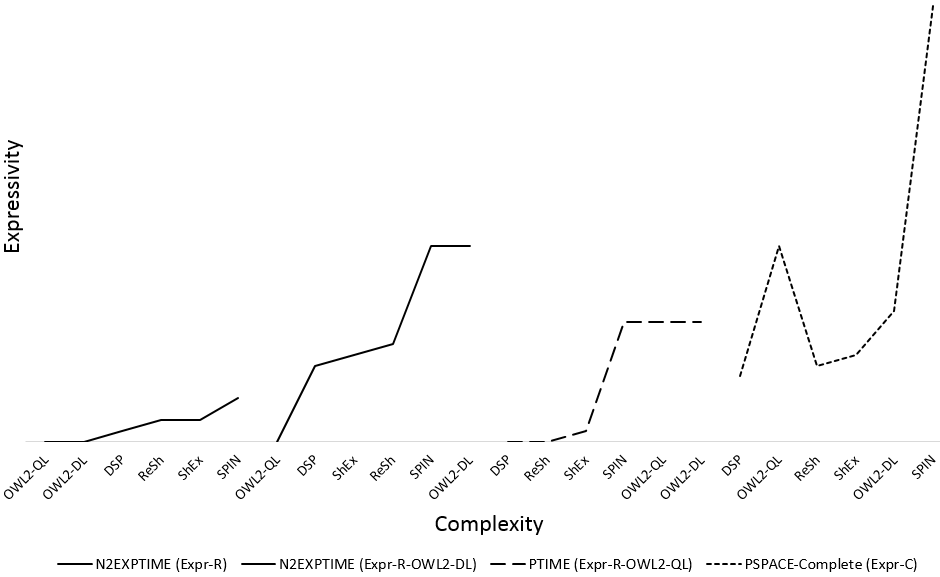
\includegraphics[width=1.00\textwidth]{expressivity-complexity-3.png}
	%\caption{Expressivity and Complexity}
	%\label{fig:expressivity-complexity}
%\end{figure}
\textcolor{red}{needs modification}

We assigned the five most promising constraint languages to two expressivity, and to four complexity classes.
Expressivity and complexity classes can be combined in a diagram (see figure Figure~\ref{fig:expressivity-complexity}).

\begin{figure}
	\centering
		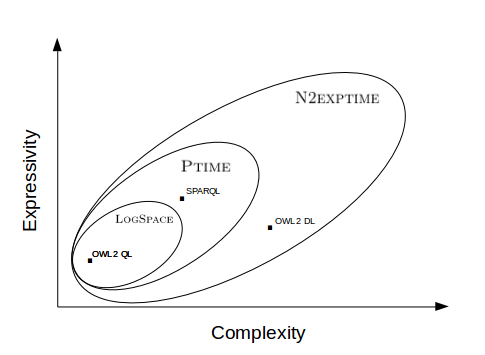
\includegraphics[width=0.95\textwidth]{complexiity_and_expressivity.png}
	\caption{Complexity and Expressivity Classes}
	\label{fig:expressivity-complexity}
\end{figure}

It depends on the individual use case, which constrains are needed to express and therefore which constraint language to choose.
%As a consequence, you may select a constraint language which is not the most expressive one within one specific expressivity class, 
%but may be better evaluated according to one or multiple user-friendliness classes.
If, for instance, reasoning should not be performed and three particular constraints should be covered by the constraint language.
Even if the absolute expressivity (\ms{Expr-C}) of SPIN is much higher than the one of ShEx (\ms{Expr-C}(ShEx) $\subset$ \ms{Expr-C}(SPIN)) 
, the relative expressivity of this expressivity class could be the same for ShEx and SPIN - in case the three constraints are covered by both.
\er{The expressivity here (in figure) is not constraint specific expressivity, it is more general. However, constraint specific expressivity must follow.}
\tb{we need to create a new figure}
%Now, the user-friendliness classes comes into play:
%\begin{eqnarray*}
%\ms{UF-L}(SPIN) \subset \ms{UF-L}(ShEx), \ms{UF-I}(SPIN) \subset \ms{UF-I}(ShEx) \\
%\ms{UF-C}(SPIN) \subset \ms{UF-C}(ShEx), \ms{UF-L}(ShEx) \subset \ms{UF-L}(SPIN)
%\end{eqnarray*}
%Although, SPIN is more adopted than ShEx, ShEx is a high-level compared to a low-level language, ShEx is more intuitive and concise than SPIN.
%According to this evaluation, tools may recommend alternatives to the most expressive language SPIN.  

\section{RDF Validation Requirements and Reasoning}
\label{sec:RDF-validation-requirements-and-reasoning}

Reasoning and validation are very closely related. 
Reasoning is the process of determining what follows from what has been
stated.  Reasoning ranges from simple (Jedi students are Jedis, Luke is a Jedi student, therefore Luke is a Jedi) to the very complex. Reasoning can
also recognize impossibilities ( Jedi masters are Jedis, Yoda is a Jedi master, Yoda
is not a Jedi, therefore there is a contradiction). 
Both should be possible: (1) validation with reasoning and (2) validation without reasoning. 
Reasoning may be a pre validation step to infer triples resolving constraint violations or to infer triples for which constraints are validated.

%Reasoning may be a pre validation step to infer triples resolving constraint violations.
%According to the existential restriction \ms{Jedi $\sqsubseteq$ $\exists$ hasJediWaepon . JediWeapon} every Jedi has at least one Jedi weapon.
%Luke is a Jedi (\ms{Jedi(Luke)}) having a blue laser sword (\ms{hasLaserSword(Luke, BlueLaserSword)}.
%As it is not defined that laser swords are Jedi weapons and as Luke is a Jedi, the existential restriction causes a constraint violation. 
%This constraint violation is not raised when we define that laser swords are Jedi weapons (\ms{hasLaserSword $\sqsubseteq$ hasJediWaepon} ) 
%and \ms{hasLaserSword} is a sub-property of \ms{hasJediWeapon} (\ms{LaserSword $\sqsubseteq$ JediWeapon}).
%
%It makes also sense to perform reasoning to infer triples for which constraints are validated.
%The existential restriction \ms{Jedi $\sqsubseteq$ $\exists$ hasLaserSword . LaserSword} forces Jedis to have at least one laser sword.
%The existential restriction is not checked for the triple \ms{YediMaster(Yoda)}, as \ms{Yoda} is a \ms{JediMaster} and not a \ms{Jedi} as well.
%If, however, our knowledge base contains the axiom \ms{JediMaster $\sqsubseteq$ Jedi}, the triple \ms{Jedi(Yoda)} is inferred and the existential restrictions is validated for the individual \ms{Yoda}, raising a constraint violation if a triple such as \ms{hasLaserSword(Yoda, GreenLaserSword)} is not included in the knowledge base. 

\subsection{OWL 2 QL Reasoning}

\textbf{Subsumption}\footnote{corresponds to R-100-SUBSUMPTION}\textbf{.}
Subsumption relationships of both classes and properties are part of basic reasoning.

\begin{center}
\begin{DL}
Jedi &$\sqsubseteq$ FeelingForce \\
JediMaster &$\sqsubseteq$ Jedi \\
\end{DL}
\end{center}

All Jedi masters are Jedis feeling the force.
These sub-class relationships can also be expressed by OWL 2 QL:

\begin{ex}
Jedi RDFs:subClassOf FeelingForce . 
JediMaster RDFs:subClassOf Jedi . 
\end{ex}

Valid data must contain the three class assignments \ms{JediMaster(Yoda)}, \ms{Jedi(Yoda)}, and \ms{FeelingForce(Yoda)}.
These class assignments can be either explicitly stated or implicitly inferred when reasoning is performed before actually validating the data.

When only the triple \ms{Yoda a JediMaster} is given and reasoning is not executed, then a constraint violation is raised.
After reasoning, however, the triples \ms{Yoda a Jedi , FeelingForce} are inferred resulting in valid data. 

\textbf{Property Domain}\footnote{corresponds to R-25-PROPERTY-DOMAIN}\textbf{.}
The property domain constraint

\begin{DL}
$\exists$ studentOf . $\top$ $\sqsubseteq$ JediStudent \\
\end{DL}

restricts that individuals having studentOf relationships must be Jedi students.
This property domain constraint can also be expressed by OWL 2 QL:

\begin{ex}
studentOf RDFs:domain JediStudent .
\end{ex}

Without reasoning, the data \ms{Anakin studentOf Obi-Wan} is invalid and causes a constraint violation, as it is not explicitly stated that \ms{Anakin} is assigned to the class \ms{Jedi}. 
When inferencing is performed before validating, the class assignment \ms{Anakin a Jedi} is inferred which prevents the constraint violation to be raised.

\textbf{Existential Quantification}\footnote{corresponds to R-86-EXISTENTIAL-QUANTIFICATION-ON-PROPERTIES}\textbf{.}

\begin{center}
\begin{DL}
Jedi $\sqsubseteq$ $\exists$ hasLaserSword . LaserSword
\end{DL}
\end{center}

Here, existential quantification let us refer to all those individuals that are connected by \ms{hasLaserSword} to an individual that is an instance of the class \ms{LaserSword}.
In OWL 2 DL, this existential quantification can also be expressed:

\begin{ex}
[ a owl:Restriction ;
  owl:onProperty hasLaserSword ;
  owl:someValuesFrom LaserSword ;
  RDFs:subClassOf Jedi ] .
\end{ex}

When our data contains the triple \ms{Luke hasLaserSword BlueLaserSword} and we perform reasoning, we can infer that \ms{Luke} is a \ms{Jedi}, as he has a laser sword.
As the individual \ms{Luke} is assigned to the class \ms{Jedi}, all constraint associated with this class are also validated, for example that Jedis must have blue laser swords.
Without reasoning, these constraints won't be validated as \ms{Luke} is not within the class extension of \ms{Jedi}.

\subsection{OWL 2 DL Reasoning}

\textbf{Universal Quantification}\footnote{corresponds to R-91-UNIVERSAL-QUANTIFICATION-ON-PROPERTIES}
contain all those individuals that are connected by a particular property only to individuals that are instances of a specific class.
Siths, e.g., can only have Siths as mentors (\ms{Sith $\sqsubseteq$ $\forall$ hasMentor.Sith}), 
which cannot be expressed by OWL 2 QL, but by OWL 2 DL \cite{owl2profiles2008}:

\begin{ex}
[ a owl:Restriction ;
  owl:onProperty hasMentor ;
  owl:allValuesFrom Sith ;
  RDFs:subClassOf Sith ] .
\end{ex}

When performing reasoning, the triples \ms{DarthMaul hasMentor DarthSidious} and \ms{DarthSidious a Sith} infer that \ms{DarthMaul} is a Sith.
When reasoning is not wished, these explicitly stated triples cause a constraint violation, as each resource having \ms{hasMentor} relationships to a Sith must also be a Sith (which is not explicitly stated in the data).

\section{RDF Validation Requirements without Reasoning}

For the majority of the requirements to formulate RDF constraints, reasoning is not related to the constraints and is therefore not needed to be performed prior to validation. 
It is also possible, however, to reason before validating constraints for which reasoning does not affect validation results.
If we do reasoning by query rewriting in terms of backward chaining and if we run a constraint validation query through an engine like the --ontop-- framework\footnote{\url{http://ontop.inf.unibz.it}} or ELITE (federated query engine) \cite{nolle2013elite}, the engine will only do some rewritings if it is possible, and if you just check e.g. pattern matching there will be no rewriting.

\subsection{Expressible by OWL 2}
\label{sec:RDF-validation-requirements-without-reasoning-2}

%\textbf{Literal Pattern Matching}\footnote{corresponds to R-44-PATTERN-MATCHING-ON-RDF-LITERALS}\textbf{.} 
%There are multiple use cases associated with the requirement to match literals according to given patterns.
%
%Luke's droids can only have the numbers "R2-D2" or "C-3PO".
%The universal restriction part of this constraint can be expressed by OWL 2 DL:
%\ms{LukesDroids $\sqsubseteq$ $\forall$ droidNumber . DroidNumber}.
%The restriction of the datatype \ms{DroidNumber}, however, cannot be expressed in DL, but OWL 2 DL can be used anyway:
%
%\begin{ex}
%DroidNumber 
    %a RDFs:Datatype ;
    %owl:equivalentClass [
        %a RDFs:Datatype ;
        %owl:onDatatype xsd:string ;
        %owl:withRestrictions ( 
            %[ xsd:pattern "R2-D2|C-3PO" ] ) ] .
%\end{ex}
%
%The second axiom defines \ms{DroidNumber} as an abbreviation for a datatype restriction on \ms{xsd:string}. 
%The first axiom explicitly declares \ms{DroidNumber} to be a datatype. 
%The datatype \ms{DroidNumber} can be used just like any other datatype like in the universal restriction above.
%The literal pattern matching constraint validates \ms{DroidNumber} literals according to the stated regular expression causing a constraint violation for the triples 
%\ms{Luke hasDroid Droideka} and \ms{Droideka droidNumber "Droideka"\textasciicircum{}\textasciicircum{}DroidNumber}, 
%but not for the triples \ms{Luke hasDroid R2-D2} and \ms{R2-D2 droidNumber "R2-D2"\textasciicircum{}\textasciicircum{}DroidNumber}.

\textbf{Allowed Values}\footnote{corresponds to R-30-ALLOWED-VALUES}\textbf{.}
It is a common requirement to narrow down the value space of a property by an exhaustive enumeration of the valid values (both literals or resources). This is often rendered in drop down boxes or radio buttons in user interfaces. 
The constraint 'Jedis can only have blue, green, or white laser swords' can be expressed by OWL 2 DL, DSP, ReSh, ShEx, SPIN, and SPARQL.
\begin{center}
\begin{DL}
Jedi $\equiv$ $\exists$ laserSwordColor . \{blue, green, white\} \\
\end{DL}
\end{center}
%In DSP, the constraint does not look that concise:
%
%\begin{ex}
%personDescriptionTemplate
    %a dsp:DescriptionTemplate ;
    %dsp:resourceClass Jedi ;
    %dsp:statementTemplate [
        %a dsp:LiteralStatementTemplate ;
        %dsp:property laserSwordColor ;
        %dsp:literalConstraint [
            %a dsp:LiteralConstraint ;
            %dsp:literal "blue" ;
            %dsp:literal "green" ;
            %dsp:literal "white"] ] .
%\end{ex}

When representing the constraint by OWL2 DL a new datatype is defined by simply enumerating its literals:

\begin{ex}
laserSwordColor RDFs:range laserSwordColors . 
laserSwordColors
    a RDFs:Datatype .
    owl:oneOf ( "blue" "green" "white" ) .
\end{ex}

Data containing the triples \ms{Yoda a Jedi ; laserSwordColor 'blue'} is valid, 
whereas data including the triples \ms{DarthMaul a Jedi ; laserSwordColor 'red'} is invalid.

\textbf{Context-Specific Exclusive OR of Properties}\footnote{corresponds to  R-11-CONTEXT-SPECIFIC-EXCLUSIVE-OR-OF-PROPERTIES}\textbf{.}
An individual can either have a relationship via property A or via property B, but not both.
To take an example, a Jedi is either attacking by sword or by force but not both (such a fight would not be fair):

\begin{center}
\begin{DL}
Jedi &$\sqsubseteq$ ($\neg$ A $\sqcap$ B) $\sqcup$ (A $\sqcap$ $\neg$ B) \\
A &$\equiv$ $\exists$ attackingBySword . xsd:boolean \\
B &$\equiv$ $\exists$ attackingByForce . xsd:boolean \\ 
\end{DL} 
\end{center}

Context-specific exclusive OR of properties can be expressed by ShEx. 
In this case, the constraint context is the class \ms{Jedi}.

\begin{ex}
Jedi { (  
    attackingBySword xsd:boolean | 
    attackingByForce xsd:boolean ) }
\end{ex}

The same constraint may be expressed by OWL 2 DL, but not very intuitively and concisely.
This can rather be seen as a workaround, as anonymous classes are built for each of the exclusive properties.

\begin{ex}
Jedi owl:disjointUnionOf ( CC1 CC2 ) . 
CC1 RDFs:subClassOf [
    a owl:Restriction ;
    owl:onProperty attackingBySword ;
    owl:someValuesFrom xsd:boolean ] .
CC2 RDFs:subClassOf [
    a owl:Restriction ;
    owl:onProperty attackingByForce ;
    owl:someValuesFrom xsd:boolean ] .
\end{ex}

Consider the triples \ms{Jedi(Luke)}, \ms{attackingBySword(Luke,true)}, \ms{Jedi(DarthSidious)},
\ms{attackingByForce(DarthSidious,true)}, and \ms{attackingBySword(DarthSidious,true)}
Luke as well as Darth Sidious are associated with the class \ms{Jedi}.
As Darth Sidious has both relationships, a constraint Violation is raised.

\subsection{Expressible by Other Constraint Languages}

The majority of constraints can neither be expressed by OWL 2 QL nor by OWL 2 DL. 
In such cases, these constraints are represented by other constraint languages like DSP, ShEx, ReSh, or SPIN.

\textbf{Default Values}\footnote{corresponds to R-31-DEFAULT-VALUES-OF-RDF-OBJECTS and R-38-DEFAULT-VALUES-OF-RDF-LITERALS}\textbf{.}
It should be possible to declare the default value for a given object and data property, e.g. so that input forms can be pre-populated and to insert a required property that is missing in a web service call. 
Siths have per default two red laser swords.
If there is only stated that Darth Maul is a Sith (\ms{DarthMaul a Sith .}), then additional default triples should be inferred: 
\ms{laserSwordColor(DarthMaul,"red")} and \ms{numberLaserSwords(DarthMaul,2)}.

The default values constraint can only be expressed by ReSh, SPIN, and SPARQL.
In SPIN, we can define a rule associated with the class \ms{owl:Thing}.
This rule is applicable for each resource, as each resource is implicitly of the type \ms{owl:Thing}. 

\begin{ex}
owl:Thing spin:rule [ a sp:Construct ; sp:text """
    CONSTRUCT {
        ?this laserSwordColor "red" ;
              numberLaserSwords 2 . }
    WHERE {             
        ?this a Sith . } """ ; ] .
\end{ex}

For each resource, the SPARQL CONSTRUCT query within the rule is executed creating the default triples.
ReSh can also be used to express default values:

\begin{ex}
Sith a ResourceShape ;
    property [
        name "laserSwordColor" ;
        propertyDefinition laserSwordColor ;
        valueType xsd:string ;
        defaultValue "red"'
        occurs Exactly-one ; ] .
\end{ex}

\section{Implementation}

SPARQL is generally seen as the method of choice to validate RDF data according to certain constraints, although it is not ideal for their formulation. 
In contrast, OWL 2 DL constraints are comparatively easy to understand, but lack an implementation to validate RDF data. However, reasoning in OWL supports the identification of inconsistencies, which is also known as ontology debugging \cite{stuckenschmidt2008debugging}. Despite the fact that inconsistency detection especially in DL has already been studied extensively, it is not sufficient for constraint validation.
Bosch and Eckert\cite{BoschEckert2014-2} use SPIN as basis to define a
validation environment in which the validation of any constraint language\footnote{the only limitation is that constraint languages must be represented in RDF} can be implemented by representing them in SPARQL. 
The validation implementation of constraint languages is fully declarative,
consisting of a mapping from a constraint language to SPIN in form of SPARQL CONSTRUCT queries.
SPIN represents both the SPIN mappings and the SPARQL queries in RDF. 
Within the validation environment, we fully implemented an automatic RDF validation of all OWL 2 DL\footnote{and therefore all OWL 2 QL constructs} constructs. 
The implementation can be tested at \url{http://purl.org/net/RDFval-demo} and
the OWL 2 SPIN mapping is maintained at \url{https://github.com/boschthomas/OWL2-SPIN-Mapping}.

The developed constraint language classification according to the three dimensions expressivity, complexity, and user-friendliness leads to many possible extensions of the RDF validator and similar validation systems.
Users may choose if they wish to execute reasoning as a pre-validation step and which reasoning axioms they want to use to express their inference rules.
They may also select which constraints they need for their use cases.

As we defined an ordering of constraint languages for each expressivity class, we assigned reasoning axioms and constraints to complexity classes, we evaluated constraint languages regarding multiple user-friendliness criteria, the validator can provide a list of constraint languages for which the expressivity is enough to express the wished constraints and axioms.
The validator can also recommend a constraint language of that list whose user-friendliness is evaluated to be the highest according to the user-friendliness criteria.
As reasoning may cause high complexity, the validator may show which axioms from the user's selection cause the determined complexity class 
and it may provide solutions how to get to the next lower complexity class.

\section{Related Work}

Tao \cite{tao2012integrity} proposed an OWL 2 DL extension to support integrity constraints and enables thereby the use of OWL as a constraint language for validation including the closed-world assumption. Beside a solution to explanation and repair of constraint violations, i.e. for integrity constraints, the author describes a sound and complete approach for constraint validation by conjunctive query answering.

Siren and Tao proposed an alternate semantics for OWL using CWA so that it could be used to validate integrity constraints.
This semantics is implemented in the Stardog database\footnote{\url{http://stardog.com/}}\cite{SirinTao2009}. 
They examined integrity constraint semantics proposed in the deductive databases literature and adopted them for OWL
by reducing the validation of integrity constraints to SPARQL query answering by means of reasoners.
This OWL semantics, however, was never submitted to a standards organization such as the W3C.

In description logics, reasoning tasks like query answering or detection of inconsistencies require the consideration of knowledge that is not only defined explicitly but also implicitly. To do so there are two different ways called forward- and backward-chaining. The first implies a materialized knowledge base, where the original knowledge base is extended by all assertions that can be inferred. State-of-the-art DL or OWL reasoners that following this approach are e.g. FaCT++ \cite{tsarkov2006fact++}, Pellet \cite{sirin2007pellet},  RacerPro \cite{haarslev2001racer}, or HermiT \cite{horrocks2012hermit}. On the second approach, the original knowledge base is kept in its original state and before queries are evaluated against the knowledge base, the queries will be rewritten such that its rewritings will consider also the implicit knowledge in the returned result set. Approaches following this way are e.g., \textsf{PerfectRef} given by Calvanese et al. \cite{Calvanese2007} or \textsf{TreeWitness} proposed by Kontchakov et al. \cite{kontchakov2011combined}. The choice between these two different ways depends on the specific application case. So the first kind is probably applied on local knowledge bases whereas the second is more appropriated for federative environments like in \cite{nolle2014efficient,nolle2013elite}.

\section{Conclusion and Future Work}

\bibliography{../../literature/literature}{}
\bibliographystyle{plain}
\setcounter{tocdepth}{1}
%\listoftodos
\end{document}
